% TEMPLATE for Usenix papers, specifically to meet requirements of
%  USENIX '05
% originally a template for producing IEEE-format articles using LaTeX.
%   written by Matthew Ward, CS Department, Worcester Polytechnic Institute.
% adapted by David Beazley for his excellent SWIG paper in Proceedings,
%   Tcl 96
% turned into a smartass generic template by De Clarke, with thanks to
%   both the above pioneers
% use at your own risk.  Complaints to /dev/null.
% make it two column with no page numbering, default is 10 point

% Munged by Fred Douglis <douglis@research.att.com> 10/97 to separate
% the .sty file from the LaTeX source template, so that people can
% more easily include the .sty file into an existing document.  Also
% changed to more closely follow the style guidelines as represented
% by the Word sample file. 

% Note that since 2010, USENIX does not require endnotes. If you want
% foot of page notes, don't include the endnotes package in the 
% usepackage command, below.

% This version uses the latex2e styles, not the very ancient 2.09 stuff.
%\documentclass[letterpaper,twocolumn,10pt]{article}
%\usepackage{usenix,epsfig,endnotes}
\documentclass{ns-article-compact}
\usepackage{amsmath}
\usepackage{amsthm}
\usepackage{algorithm}
%\usepackage{algorithmic}
\usepackage{algpseudocode}
\usepackage{caption}
\usepackage[utf8]{inputenc}

\usepackage{wasysym}
\usepackage{xspace}
\usepackage{balance}

\usepackage{color}
\usepackage{mathrsfs}
\usepackage{multirow}
\usepackage{array}
\usepackage{verbatim}
\usepackage{graphicx,subcaption}
\usepackage{comment}
\usepackage{epsfig}
\usepackage[hyphens]{url}
\usepackage{hyperref}
\usepackage{tabularx}

\newcolumntype{Y}{>{\centering\arraybackslash}X}

\begin{document}

%don't want date printed
\date{}

\newcommand{\squishenum}{
   \begin{enumerate}
    { \setlength{\itemsep}{0pt}      \setlength{\parsep}{1pt}
      \setlength{\topsep}{1pt}       \setlength{\partopsep}{0pt}
      \setlength{\leftmargin}{1.0em} \setlength{\labelwidth}{1em}
      \setlength{\labelsep}{0.5em} } }

\newcommand{\squishlist}{
   \begin{list}{$\bullet$}
    { \setlength{\itemsep}{0pt}      \setlength{\parsep}{3pt}
      \setlength{\topsep}{3pt}       \setlength{\partopsep}{0pt}
      \setlength{\leftmargin}{1.0em} \setlength{\labelwidth}{1em}
      \setlength{\labelsep}{0.5em} } }

\newcommand{\squishlisttwo}{
   \begin{list}{$\bullet$}
    { \setlength{\itemsep}{0pt}    \setlength{\parsep}{0pt}
      \setlength{\topsep}{0pt}     \setlength{\partopsep}{0pt}
      \setlength{\leftmargin}{1em} \setlength{\labelwidth}{0.5em}
      \setlength{\labelsep}{0.5em} } }

\newcommand{\squishend}{
    \end{list}  }

\newcommand{\squishenumend}{
    \end{enumerate}  }

\newcommand{\tightcaption}[1]{\vspace{-12pt}\caption{{\bf \small #1}}
\vspace{-7pt}
}

\newcommand{\eat}[1]{}

\urlstyle{rm}

%space saving macros
\newcommand{\ispace}{\vspace{-0.08in}}
\renewcommand{\ispace}{}
\newcommand{\jspace}{\vspace{-0.06in}}
\renewcommand{\jspace}{}

\newcommand{\willgo}[1]{}
\newcommand{\TBD}[1]{[{\bf{TBD:}} #1]}
\newcommand{\tbd}[1]{[[[{\bf{TBD:}} #1]]]}
\newcommand{\todo}[1]{{\color{red} #1}}
%\newcommand{\todo}[1]{}
\newcommand{\rmv}[1]{\footnote{{\bf{CUT:}} #1}}
\newcommand{\shorten}[1]{#1}

\newcommand{\mypara}[1]{
%\smallskip
\noindent
{\bf {#1}}~}
%\renewcommand{\paragraph}[1]{{\bf #1}}
%\setlength{\textfloatsep}{10pt}
%\setlength{\floatsep}{10pt}
\newcommand{\myred}[1]{{\color{red} {#1}}}
\newcommand{\mycomment}[1]{\textit{\color{blue} {#1}}}

%\setlength{\tabcolsep}{4pt}
\newcommand{\paraspace}{\vspace{0.02in}}
\newcommand{\parab}[1]{\paraspace\noindent{\bf #1} }
\newcommand{\parae}[1]{\paraspace\noindent{\em #1} }
\newcommand{\parabe}[1]{\paraspace\noindent{\bf \em #1} }

\newcommand{\system}{{\sc Pando}\xspace}
\newcommand{\pman}{Placement Manager\xspace}

%make title bold and 14 pt font (Latex default is non-bold, 16 pt)
\def\papertitle{ Memoization of Browser Computations for a Faster Mobile Web}

\title{\papertitle}
\author{
  {\rm Ayush Goel}
  \and
  {\rm Matthew Furlong}
  \and
  {\rm HyunJong (Joseph) Lee}
}
\maketitle

% Use the following at camera-ready time to suppress page numbers.
% Comment it out when you first submit the paper for review.
\thispagestyle{empty}

\section{Introduction}
\label{sec:intro}

Page Load Time (PLT) of a website is a key performance metric that
significantly impacts user-experience, as pointed out by many recent studies
from both academia and industry~\cite{bhatti2000integrating, bouch2000quality}.
User-experience in web browsing is directly correlated to companies' revenues:
Amazon shows that reducing 100ms in PLT results in 1 percent revenue increase
and Shopzilla reports that improving PLT from 6 to 1.2 seconds increased the
revenue by 12 percent~\cite{url3}. 

There have been many prior works in improving webpage's PLT of mobile devices,
ranging from offloading computation and network tasks to
proxies~\cite{netravali2015mahimahi, sivakumar2014parcel, wang2014speedy} to
re-prioritising requests at client side by letting the client itself discover
all resources on a page~\cite{butkiewicz2015klotski, netravali2016polaris}.  It
is worthwhile to note that existing works attempt to surrogate web-tasks of
mobile devices from resource-rich server
environment~\cite{ruamviboonsuk2017vroom}.
 
The end-to-end PLT for many webpages is far from the ideal: an order
of tens of seconds on mobile devices~\cite{wang2013demystifying} and
order of seconds on stationary desktops.  Many existing solutions
often require server-side modification, which strongly discourages
content providers to use new solution. 
% Joseph: why doing at server-side is bad?
Whereas a client side solution would be agnostic of the content
provider/server that is being used to render the web pages and
optimize page load times for all web pages alike. 
Most of the existing work on client side talks about efficient ways to
optimise web cache~\cite{wang2014much}.  
Prior work shows how computation latency is the driving factor behind
large web page load time, as compared to network
latency~\cite{vesuna2016caching}.

In this work, we propose PLT optimization technique that caches output
from previous code execution of a webpage (e.g., Javascript, inline
HTML, css) on mobile devices to reduce user-perceiving PLT in exchange
of prevalent mass-storage.
Prior techniques have gone as far as caching the compiled code either
on the client side or on the server side to save on the compilation
time when the web content remains unchanged~\cite{wang2014much}. We
take this a step further, and cache the output of the execution of all
the code on a web page. ( Note that I use the word code, to
distinguish it from other components of a webpage which include layout
and data). Recent work has shown that most of the webpages remain
unchanged over a large period of time. For content-rich pages, the
amount of updates vary across Web pages. In the best (worst) case,
20\% (75\%) of the HTML page is changed over a month. Most changes are
made to data (e.g., links to images, titles) while little is made to
layout and code~\cite{wang2014much}.  This implies that most of the
code output could be reused, essentially eliminating code execution
time from the critical path of a web page load. This would bring down
the entire page load time to the time taken in rendering/painting the
layout. 
Caching the computation as a technique to optimize the execution time has
already been explored at a data center level~\cite{gunda2010nectar} and it has
shown tremendous improvement with more than 35\% job benefiting from caching.
We are trying to apply a similar technique however on the client side at a
browser level. 

\begin{figure*}[!bth]
\begin{subfigure}[h]{0.5\textwidth}
\centering
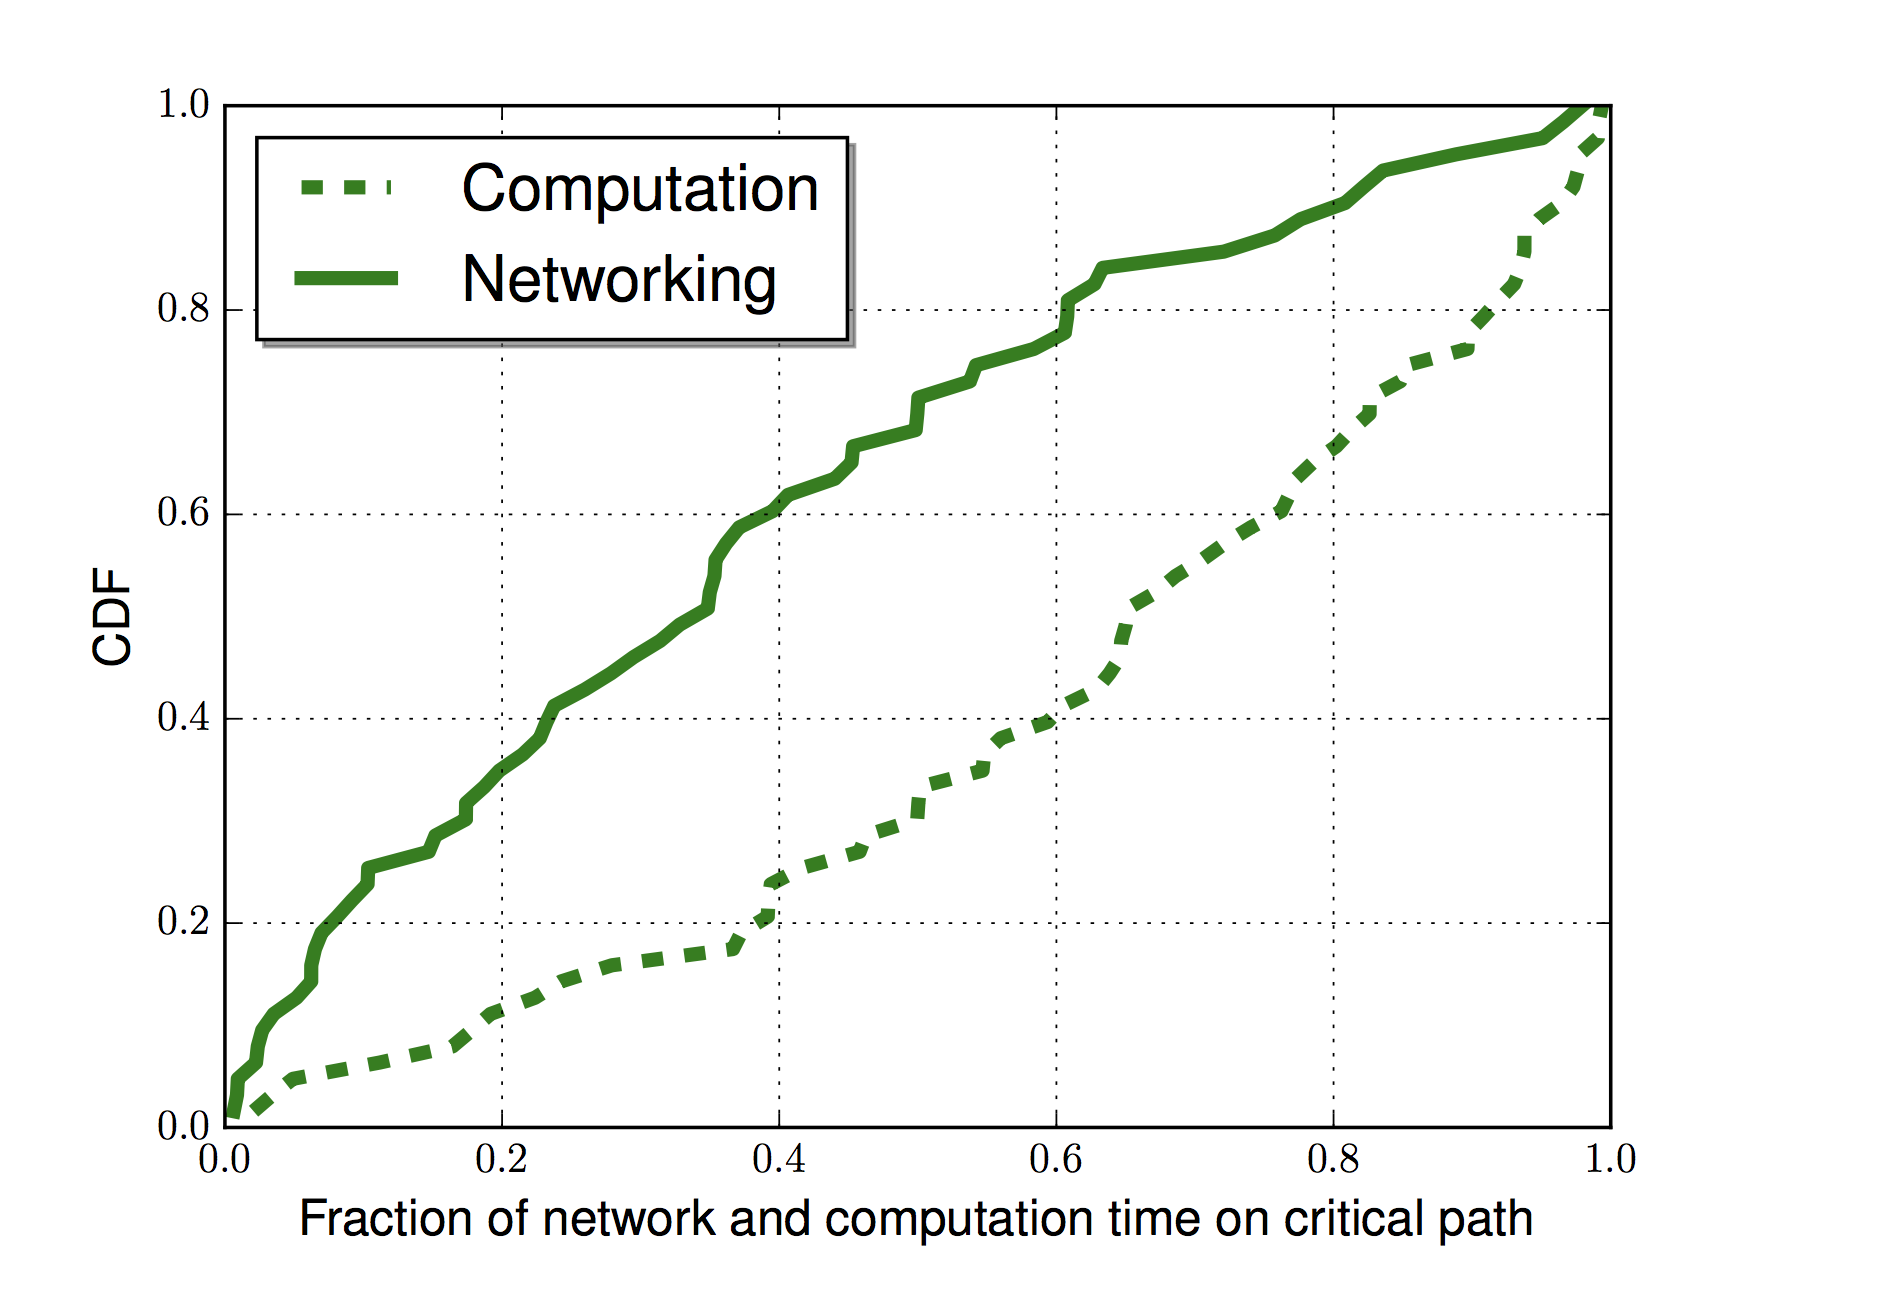
\includegraphics[width=\linewidth]{figs/comp_net.png}
\caption{Runtime information on mobile devices}
\label{fig:mobile-runtime}
\end{subfigure}
\begin{subfigure}[h]{0.5\textwidth}
\centering
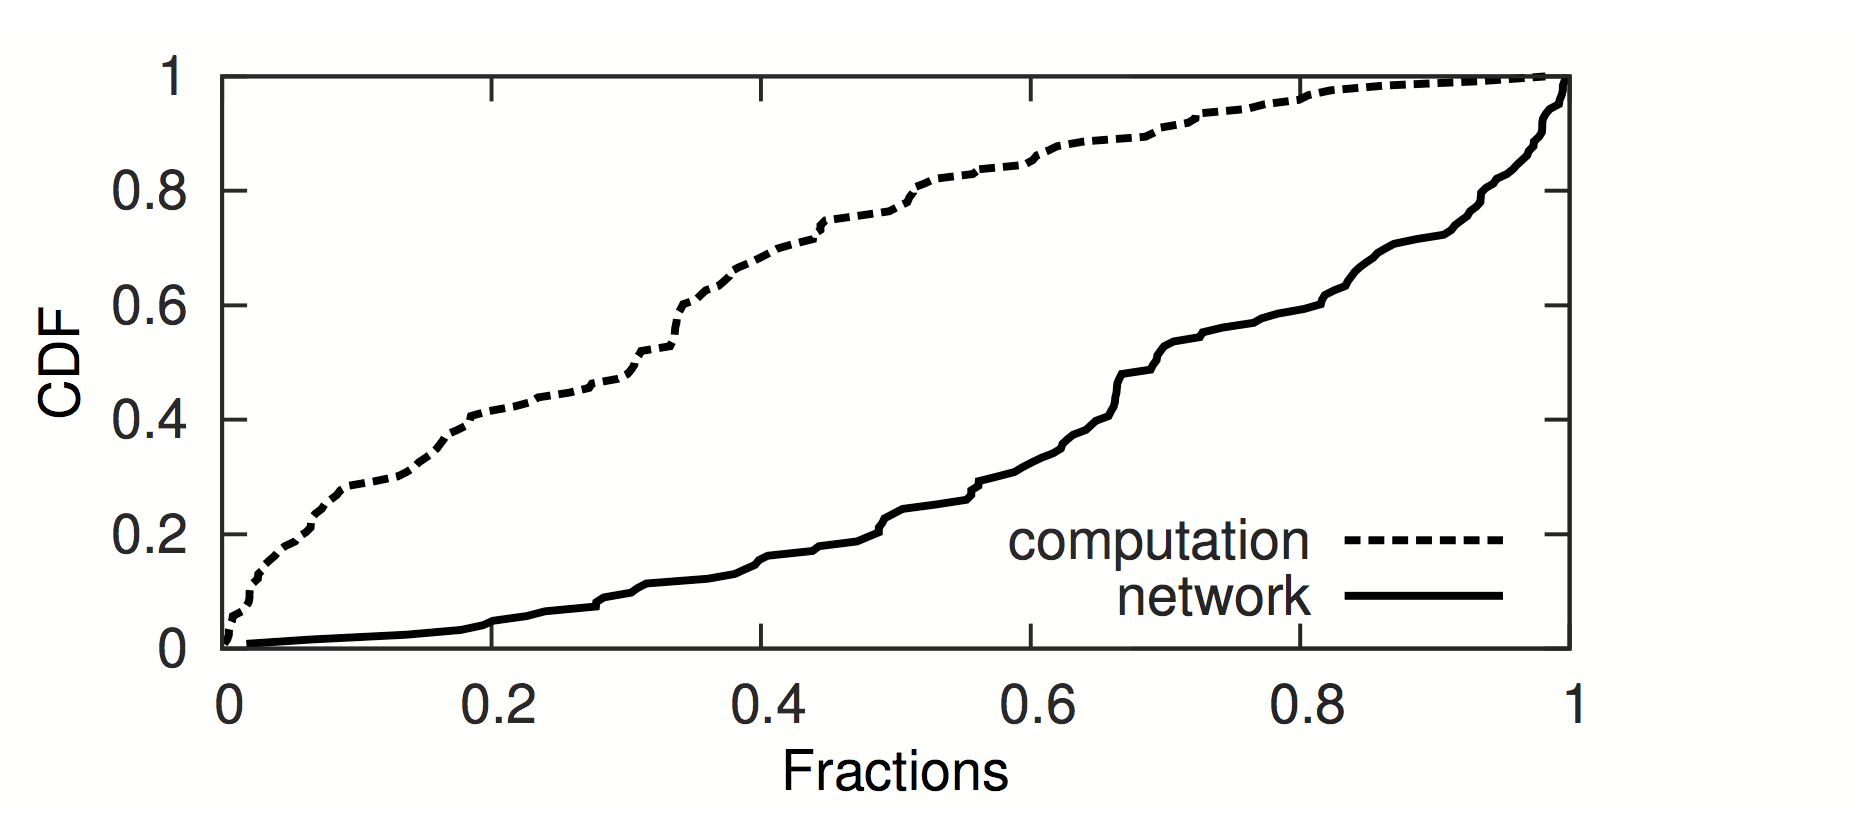
\includegraphics[width=\linewidth]{figs/comp_net_desk.png}
\caption{Runtime information on desktops}
\label{fig:mobile-runtime}
\end{subfigure}
\caption{{\color{red}Figure 1 captioon placeholder}}
\end{figure*}


\section{Motivation}
\label{sec:motivation}

% Recent effort from industry has been focused on 
% Major web browsers like Chrome, Firefox, and Safari have recenlty invested a lot of resources,
% time and energy into improving web performance on mobile devices, specifically by targeting 
% the network usage. However, the network now comprises less than 30\% \cite{njait2016www} of the total critical
% path for an average page load on a mobile device. 
% This includes caching almost 95\% of the
% resources that are fetched from the server \cite{vesuna2016caching}, dns presolution, dns caching, tcp reconnect etc.
Chrome released a paper last year showing how improved caching algorithms, despite having 
Recent effort from industry to improve mobile web performance has been
focused on reducing network usage, under assumption that network is
dominant factor in PLT. However, recent study~\cite{njait2016www}
shows that the network latency composes of less than 30\% of the total
PLT. The authors note that not only the performance of mobile network
improved but also numerious optimizations (e.g., resource
caching~\cite{vesuna2016caching}, DNS presolution and caching, TCP
Fast reconnection) contribute to reduce the network latency.
% significant improvements on the desktop, don't have the same proportionate improvements 
% on mobile devices. This is primarily attributed to the fact that computation comprises more than 65\%
% of the critical path during a page load. This illustrates the need to further optimize the computation 
% time. 


During the Chrome dev summit this year, their team announced the latest improvements they have 
made in their browser to improve the page load time. Interestingly, most of their work focuses on
improving the compilation and parsing time by introducing compile and parser cache. 
Recent studies \cite{url4} still report that the median page load time for a mobile website 
is about 14 seconds. Research \cite{url4} shows that a user will only wait for 3 seconds 
before abandoning a web site if it shows no response at all. A lot of prior work \cite {njait2016www}
has been done to compare the page load times on mobile vs desktop, and recent results
from 2016 claim that despite the increasing compute resources in mobile devices,
the computation time on mobile is significantly higher than their desktop counterparts. 
 Our experiments
on the most popular news and sports websites on the latest mobile hardware and the latest 
Chrome version reveal that despite these recent efforts, scripting still takes significantly more
time ,as compared to the other components of the total computation time. With our understanding of 
computation being the current bottleneck for high page load times, 
we conduct a set of experiments to evaluate the reasons for this
exceedingly high computation time. In order to do this, we break down computation
into four categories: scripting, loading, painting, and rendering.
and observe that scripting essentially takes more than 70\% of the total
computation time which is more than all the other categories combined (Figure 3). 
This makes it all the more important to do an in-depth analysis of the computation time to clearly
understand where exactly this time is being spent. Using results from this study, we would eventually
design our caching framework for the javascript execution output. 

\section{Design}
\label{sec:design}

\begin{figure}[t]
\centering
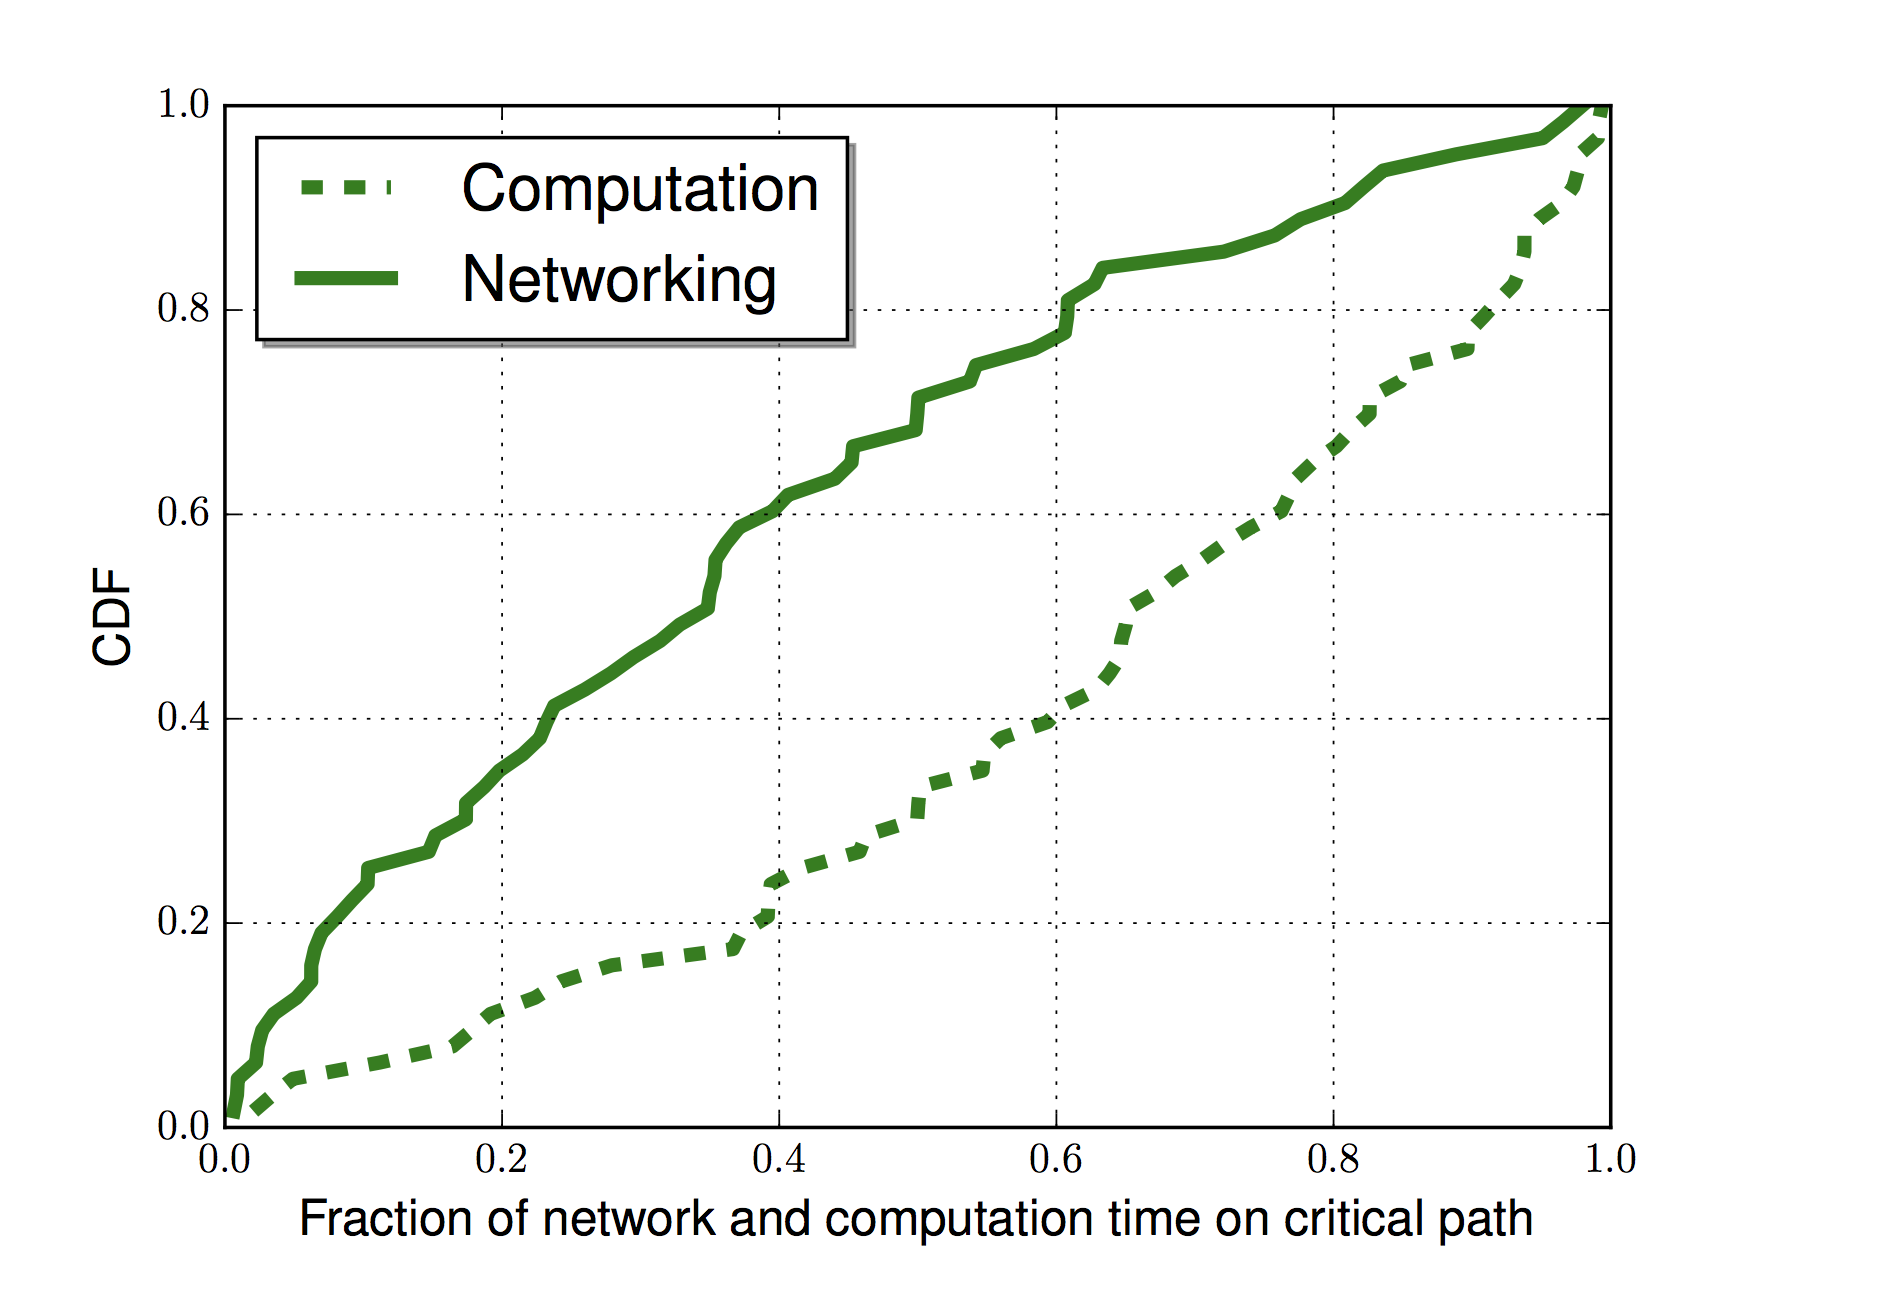
\includegraphics[width=0.9\columnwidth]{figs/comp_net.png}
\tightcaption{Runtime information on mobile devices}
\label{fig:mobile-runtime}
\end{figure}

\begin{figure}[t]
\centering
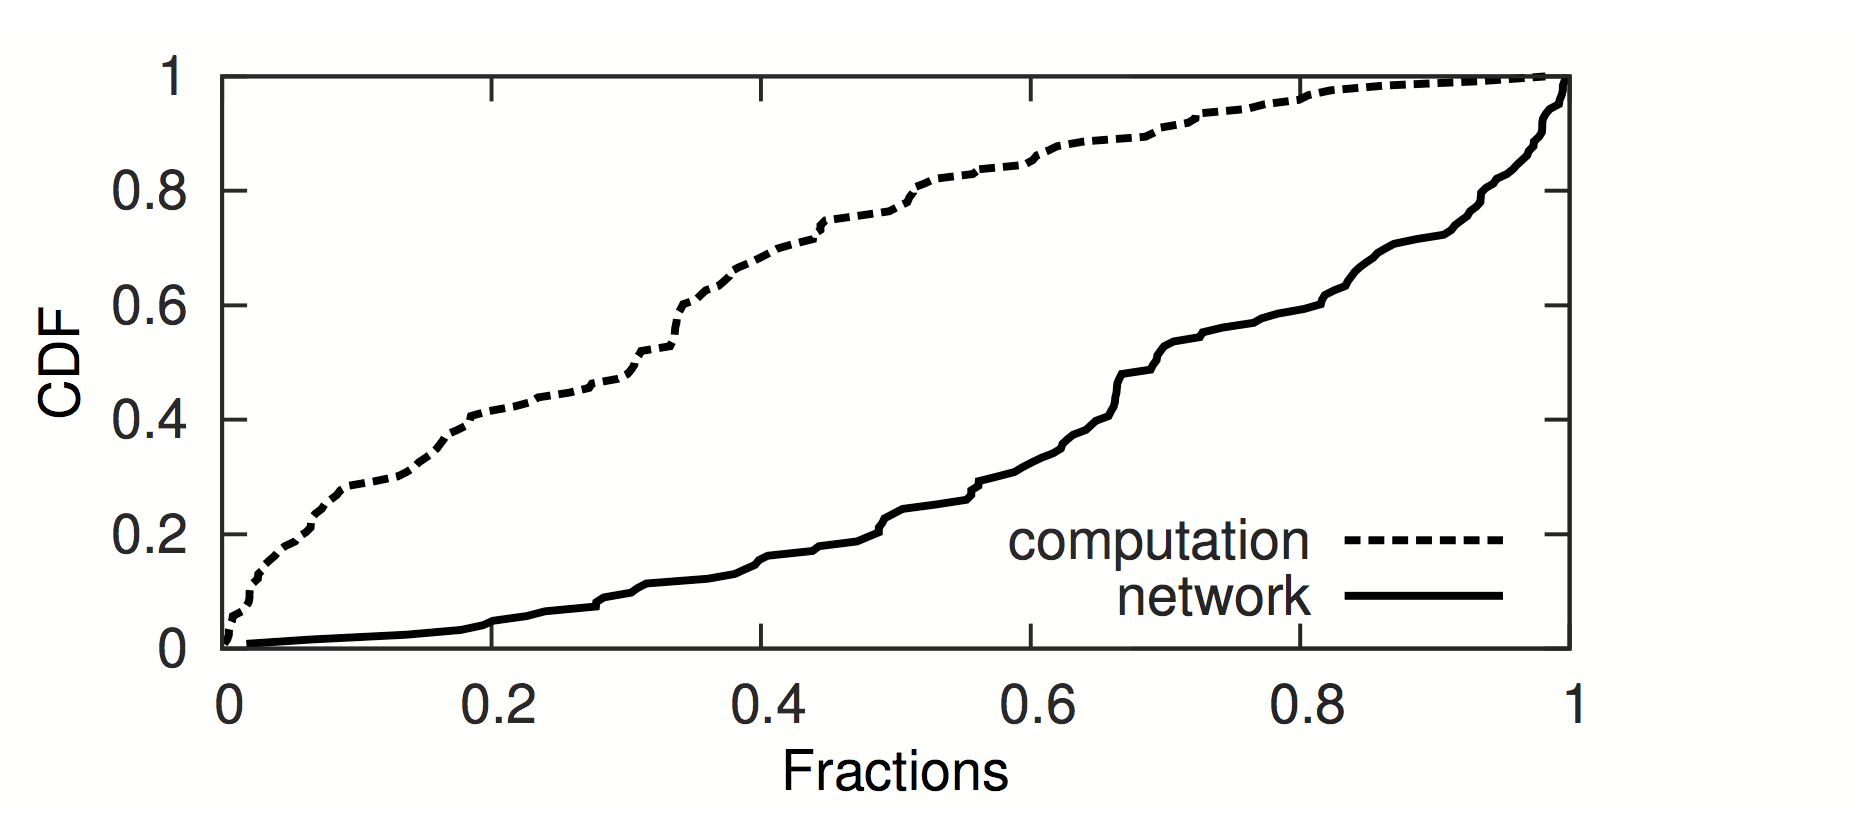
\includegraphics[width=0.9\columnwidth]{figs/comp_net_desk.png}
\tightcaption{Runtime information on desktops}
\label{fig:mobile-runtime}
\end{figure}

% \begin{figure}[t]
% \centering
% \begin{tabular}{cc}
% 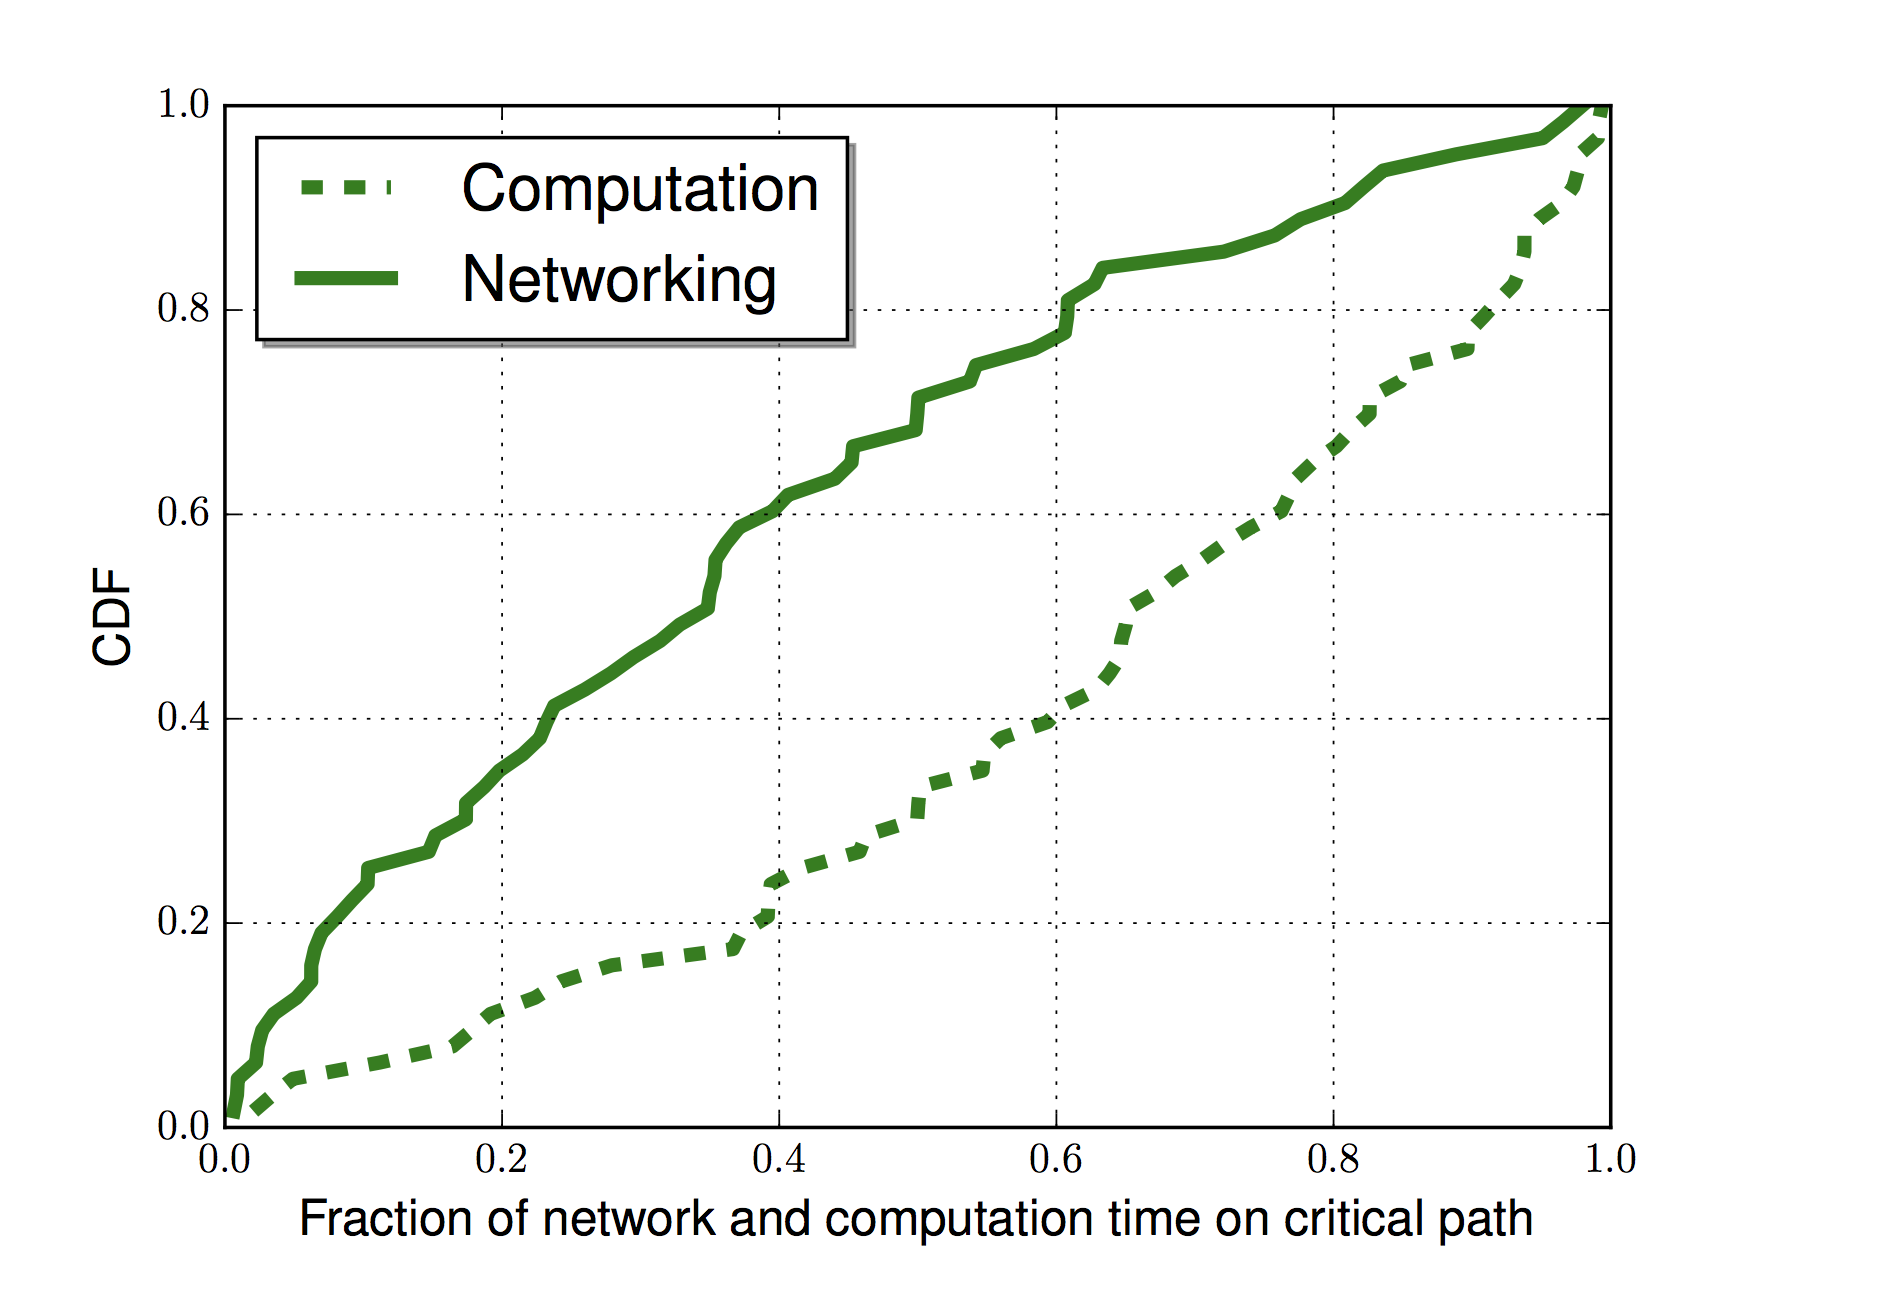
\includegraphics[width=0.9\columnwidth]{figs/comp_net.png}&
% 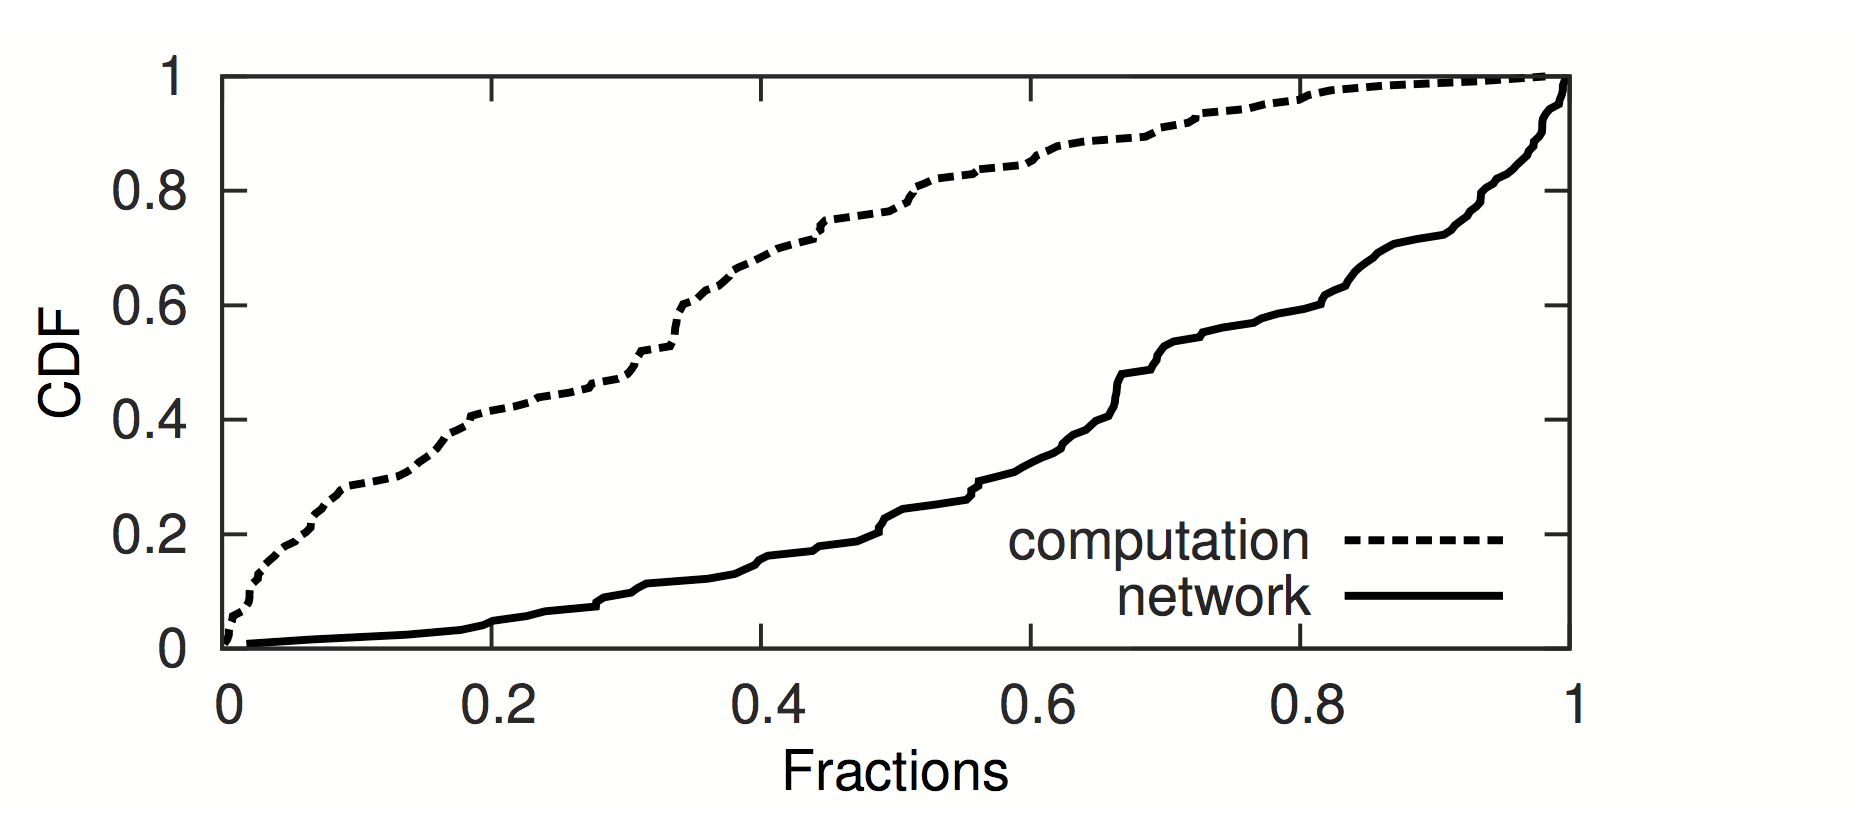
\includegraphics[width=0.9\columnwidth]{figs/comp_net_desk.png}\\
% {\small (a) Azure} & {\small (b) AWS}
% \end{tabular}
% \label{fig:dcs-local}
% \end{figure}

We propose a new technique to improve the page load time by reducing the javscript time. %Which part of the javascript time here? 
In order to do this, we intend to build a new caching framework for the modern web browsers,
specifically Google Chrome. We choose to focus on Chrome because it accounts for about 50\% of the market share in terms of browser
usage. Our caching framework will store the javascript execution result. This can mean a lot of things
due to the dynamic nature javascript. Most of the times it is simply the return value of the 
javascript functions. At other times it can be a modified DOM structure or just some intermediate result which
will be further processed by other javascript functions, later down the execution timeline. 
The expiry of this javascript exectution cache is supposed to be same as the expire of the javascript source cache. % I don't understand what this sentence means but it may be right?
There are a lot of caveats to this approach, and in our work we will explore all of these. % Again, this is really vague and I don't really understand what this means...
The biggest challenge when developing a new caching framework is modifying the current browser's code 
in order to evaluate the efficacy of our caching framework. Since a lot of browsers already implement caching
at the javascript runtime level, such as compiler and parser caches, a lot of this architecure can be borrowed
for the execution cache as well. 
Another potential challenge will be the memory overhead. Most of the popular websites which spend about 70\% 
of their time on javascript execution are running 1000s of javascript functions. Saving the output of all 
of these functions will add extra memory overhead to current browsers. 

\section{Progress}
\label{sec:Progress}


\begin{figure}[t!]
\centering
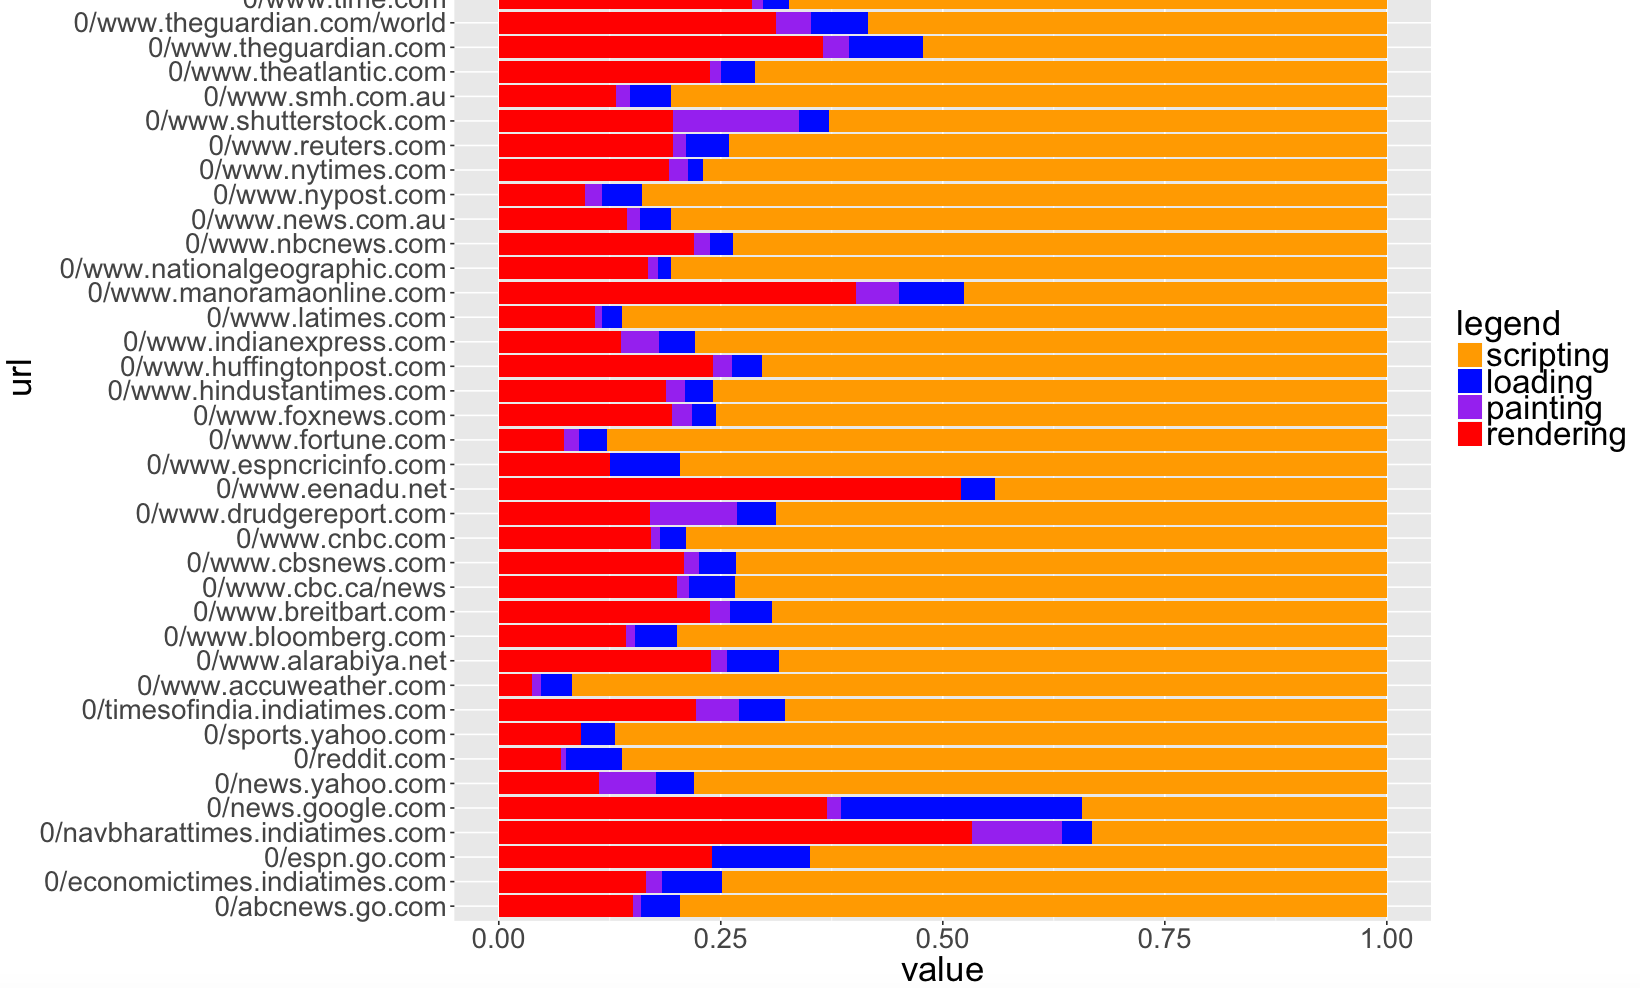
\includegraphics[width=0.99\columnwidth, scale=2.0]{figs/comp_1.png}
\tightcaption{Breakdown of computation on pixel 2}
\label{fig:act_p2}
\end{figure}

As a preliminary step in research, we first established a corpus of the top
75 news and sports websites on which we would run our experiments
in order to cater to the most popular and compute intensive websites. 
These websites are taken from the Alexa top website list.
We ran all our experiments on a Google Pixel 2. We used Chrome v 61 to run all of our experiments on the mobile device. We leveraged chrome developer tools in order
to capture the runtime traces, both for network and compute. We then analyzed these runtime
traces to draw insight into the critical path of the website, the total time being spent on the 
compute vs the total time being spent on the network, and most importantly the finer
level breakdown of the computation time to understand the true nature of computation on mobile
devices. 

We categorised computation time into four categorires, scripting, loading, rendering and
painting. Scripting is the total time being spent on
compiling, evaluating and executing javascript. Loading consists of parsing the html and css, which happens 
immediately after the payload for the network requests are received by the browser. Loading
takes these payload objects and parses them before converting them to a DOM tree. Once the DOM tree is built,
the rendering engine converts this DOM tree into a render tree, which contains the
exact coordinates and the shape of each of the DOM node. This process comrpises the rendering time of the web page.
Painting time is the time taken to process the render tree, and convert
each pixel into a bitmap.
Figure 3 shows the computation break down for these first level of categories
for the Google Pixel 2. We further break down this time into the finer level events
which are returned by Google Chrome's trace and then group them by their event name.

\begin{figure}[t!]
\centering
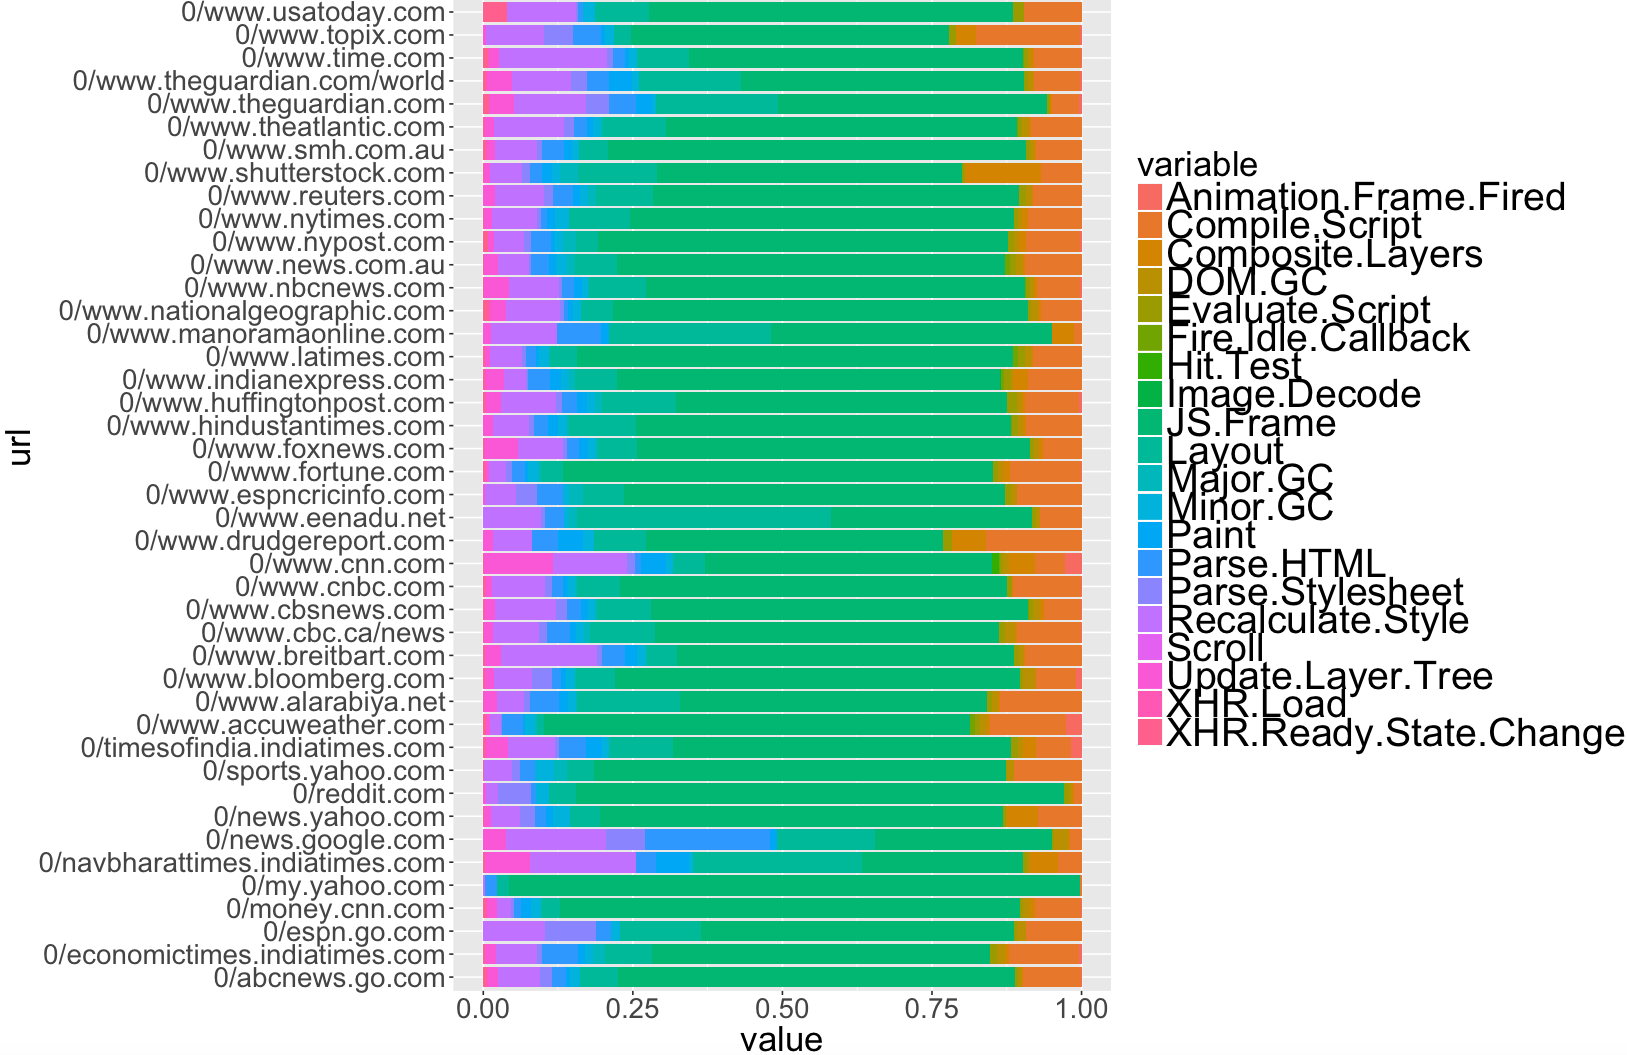
\includegraphics[width=0.9\columnwidth]{figs/comp_2.png}
\tightcaption{Breakdown of computation into finer events on pixel 2}
\label{fig:cat_p2}
\end{figure}


These results are extremely coherent with our design of implementing a javsvcript chrome
caching mechanism and show the possibility of a large improvement in the total page
load due to the high percentage share of execution time as seen in Figure 4. 

\begin{figure}[t]
\centering
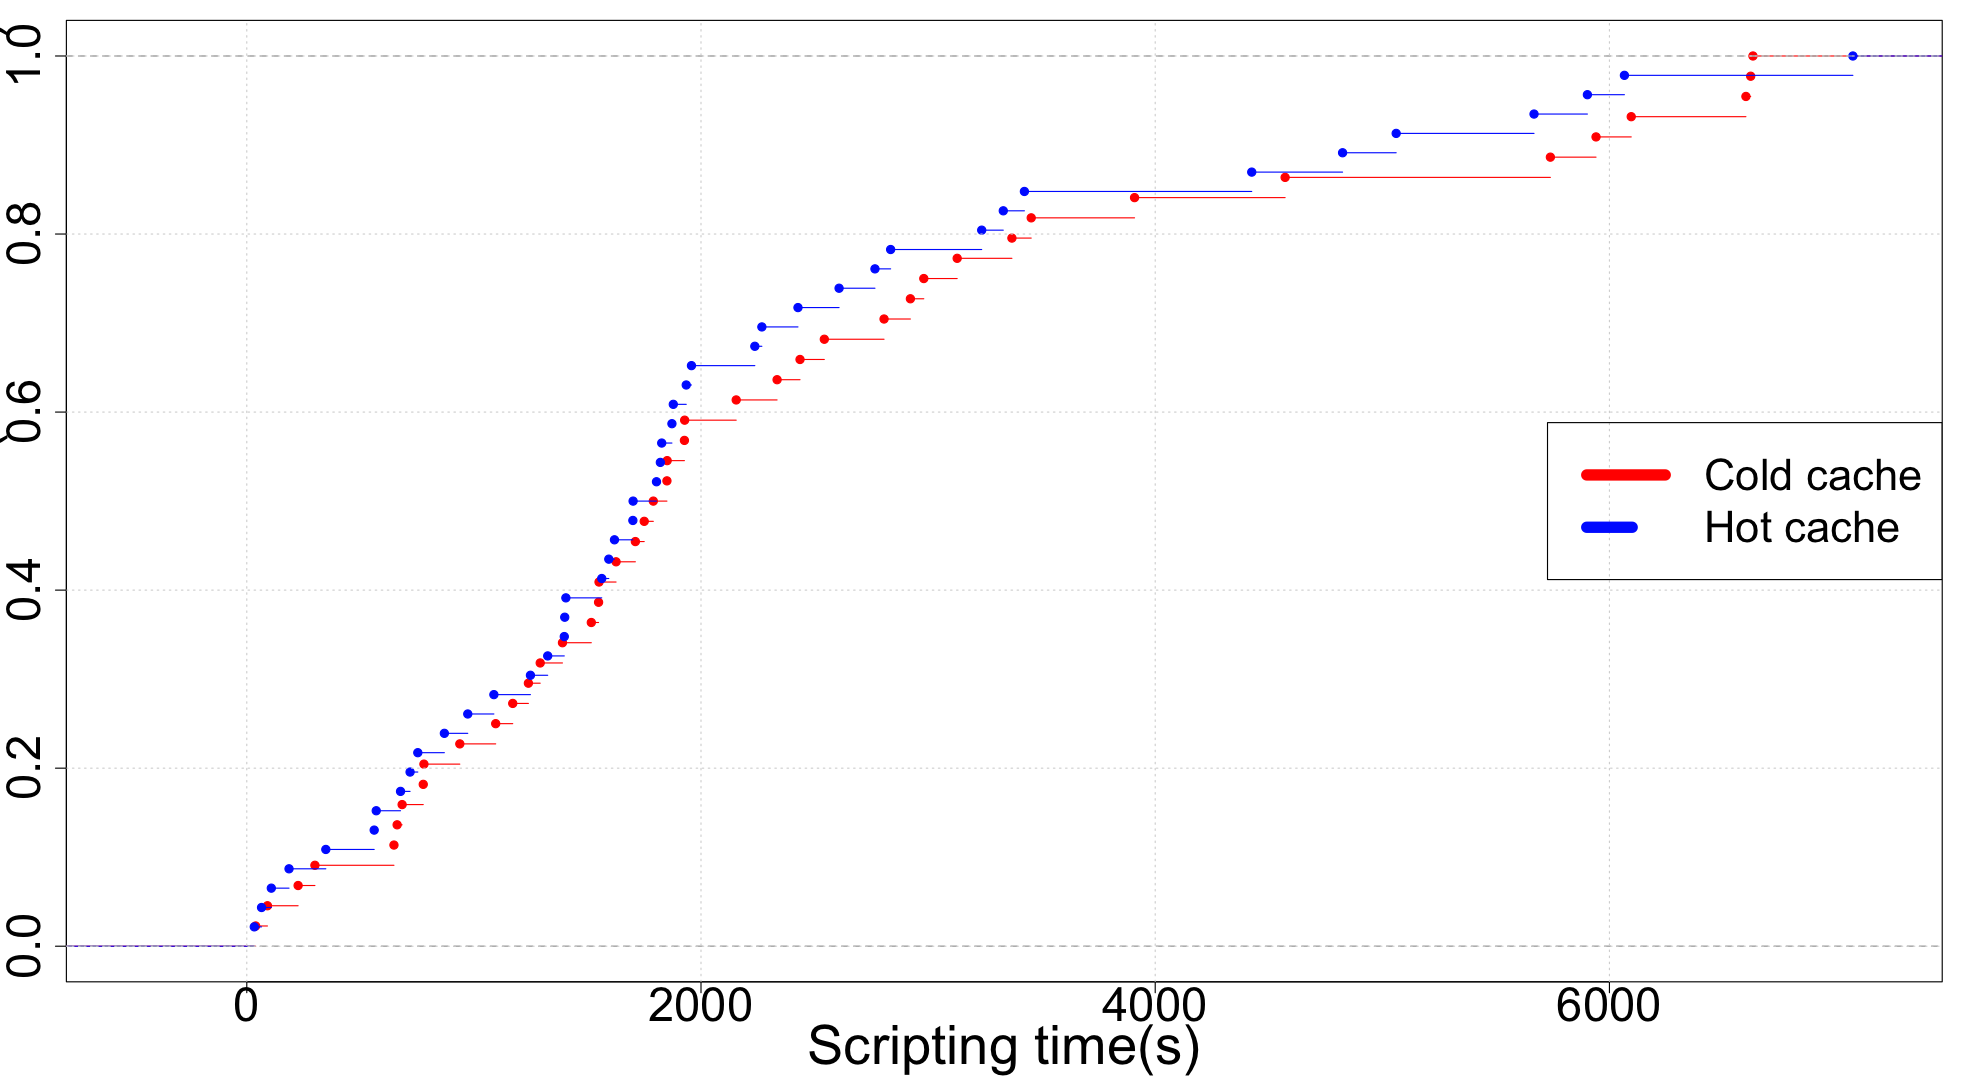
\includegraphics[width=0.9\columnwidth]{figs/chrome_script.png}
\tightcaption{CDF of scripting time with and without chrome's optimisations}
\label{fig:scripting_p2}
\end{figure}

Recently in their 2017 dev summit, the Chrome team discussed the various optimisation techniques
they have employed in the latest Chrome browser to improve the total page load time.
We did a comparison of the total page load time with and without Chrome's optimizations to see
the improvements. In order to do this, we captured the trace from Alexa's top 75 
news and sports website once with a fresh cache, ie cold cache, and then subsequently with a hot
cache which contains all of Chrome's optimizations, including its compiler and parser cache. 
As we can see from Figure 7, there has been a significant reduction in the overall compilation
time, with about 100ms reduction in median compile time. This is primarily due to the introduction of compiler and parser cache. 
The line corresponding to Cold cache refers to the fresh load of all the websites,
whereas the line corresponding to the Hot cache refers to the subsequent load
which makes use of Chrome's caching framework. 
This is also reflected partially in the overall scripting time
as shown in Figure 5. Note that scripting time is the sum of compilation, execution and other
minor javascript events in the execution pipeline like garbage collection. 
However the interesting thing to note, is that despite all these optimizations,
we observe almost neglible improvement in the median execution time of the javascript, as
shown in Figure 6. This serves as a huge motivation for the vast potential in
improving the overall page load time, by optimizing the javascript execution
time.

\begin{figure}[t]
\centering
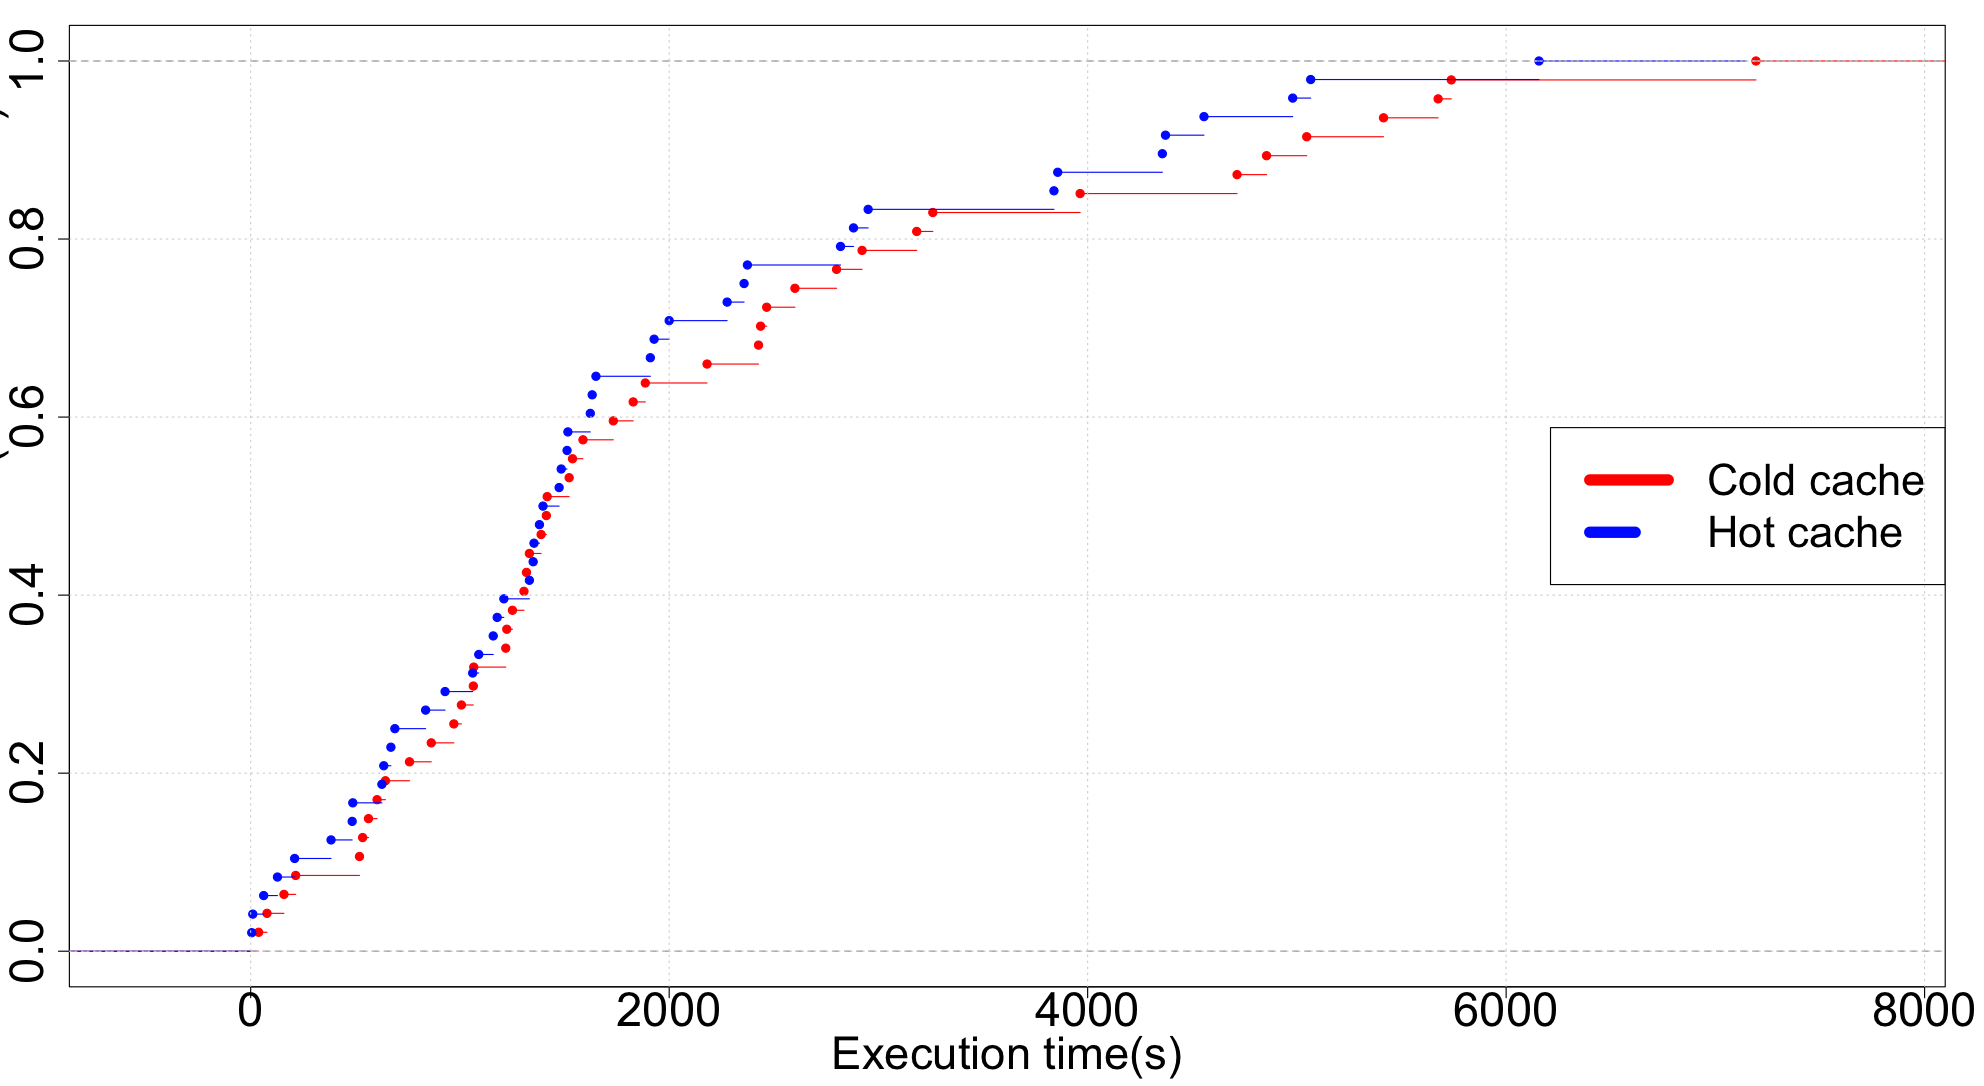
\includegraphics[width=0.9\columnwidth]{figs/chrome_exec.png}
\tightcaption{CDF of total execution time with and without chrome's optimisations}
\label{fig:compile_p2}
\end{figure}

\begin{figure}[t]
\centering
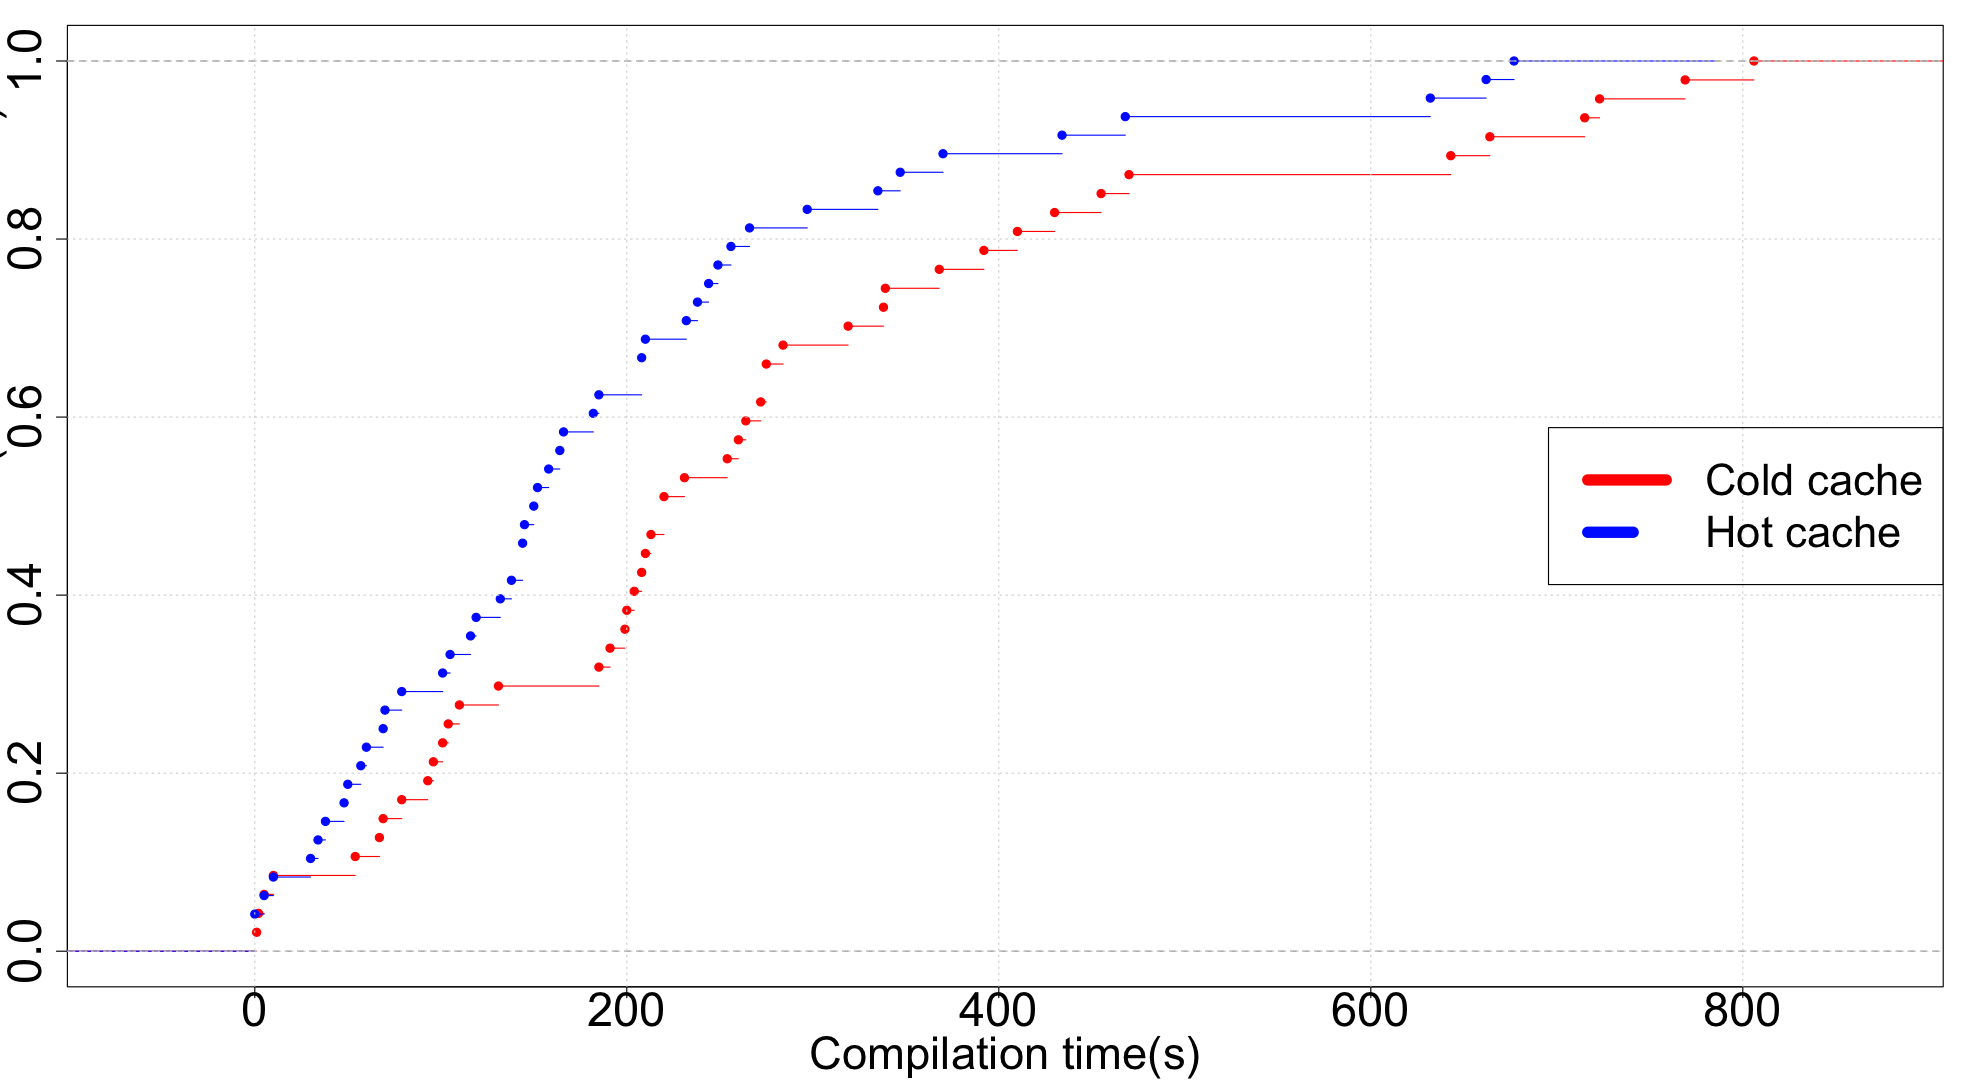
\includegraphics[width=0.9\columnwidth]{figs/chrome_compile.png}
\tightcaption{CDF of compilation time with and without chrome's optimisations}
\label{fig:compile_p2}
\end{figure}


\section{Related Work}
\label{sec:related}

Many prior works~\cite{erman2013conext, quian2012mobisys,
sivakumar2014conext, mai2012hotpar, meyerovich2010www, zhu2013hpca}
in the domain of improving web performance have been
done, ranging from optimizing webpage to reducing network time.
Recent works~\cite{vesuna2016caching, agababov2015nsdi,
butkiewicz2015usenix} propose improving computation time to further
reduce PLT.

Recent studies~\cite{erman2013conext, quian2012mobisys,
vesuna2016caching} show that computation time is major component in
PLT of mobile browsers.  Erman et al.~\cite{erman2013conext} has shown
that unlike desktop browsers, optimizations such as SPDY/HTTP2 do not
improve PLT on mobile browsers. The authors show that this is because
of the negative interactions between the cellular state machine and
the transport protocol.  Similar to our study, Qian et
al.~\cite{quian2012mobisys} argue that caching resources does not
contriute to reduction in PLT for mobile devices. Furthermore, A
recent study~\cite{vesuna2016caching} shows that how there is very
little improvement to the overall page load time despite significant
improvements in the cache hit rate. 

On contrast to, the research on explicitly improving mobile browser
performance has seen mixed results.
FLywheel~\cite{agababov2015nsdi} is Google's compression proxy that compresses web content to significantly 
reduce the use of expensive cellular data. The authors note that while Flywheel succeeds in
reducing the data usage, its effect on page load time is more mixed; it helps
the performance of certain pages and hurts the performance of others.
Flexiweb~\cite{singh2015mobicom} is built over
Google's compression proxy to ensure that the proxy does not hurt page load times. However, FlexiWeb
is not designed to explicitly improve page load performance. Wang et
al.~\cite{wang2013demystifying} show that
speculative loading in one of only client only approaches that can improve mobile
browser performance. However, speculative loading requires knowledge of what objects are likely
to be requested by the user. 


Other research works have looked at metrics that are orthogonal to the
page load time metric. Parcel~\cite{sivakumar2014conext} uses a proxy
approach to divide the page load process between the mobile device and
the proxy. Because Parcel is a network approach, the evaluations are
primarily focused on the reduction of network latency.
Klotski~\cite{butkiewicz2015usenix} focuses on increasing the number
of objects rendered in the first 5 seconds to improve the user quality
of experience. 

Other client side improvements reduce energy usage and computational
delays using parallel browsers~\cite{mai2012hotpar, meyerovich2010www}
and improved hardware~\cite{zhu2013hpca}.  By improving the
parallelization for necessary page load tasks, such as rendering,
these systems reduce energy usage and have a positive impact on page
load times. 

% While there have been several recent efforts on improving mobile browser performance
% they have not been uniformly successful due to their various limitations.


\section{Future work}
\label{sec:future-work}

Most of the project up till now has been to serve as a motivation for building 
a caching framework for the Javascript execution output. All of our experiments
have shown the positive benefits of a caching framework. 
We also have established an upper bound on the posible decrease in the page load time
in the best case scenario. 

The actual implementation of the caching framework will be our next step. 
This is more like an engineering effort, which will determine the efficacy
of our idea when we can fully evaluate the sytem. 
In order to do this, we will have to modify the production level 
source code of the Chrome browser. 

Our understanding of the current caching framework for compiler
and parser cache can be used as a reference for our Javascript caching
framework. 


\section{Contribution}
\label{sec:contribution}

Our work had a fair distribution among the three co authors. 
This being the main research project of Ayush Goel, he was primarily 
responsible for setting up the testbed for the experiments and conducting them. 
All the code for the different analysis done for the page loads, like network
analysis, trace analysis and capturing the window object state and running
a simple diff algorithm is written by Ayush Goel. He has studied the current 
optimizations in place done by Chrome, and evaluated the improvement in the
loading time with these optimizations enabled. 

Matthew Furlong, the second co author has contributed in finding 
the javascript libraries we currently use to capture the network
and time line trace for each web page load, on top of which most of 
our other analysis code is written. He has contributed in analyzing
data from our experiments by building CDFs of the results and 
comparing them with each other. 

Hyunjong Lee, the third co author has contributed in writing the mid semester
and the final reports, generating figures and writing the content. 

Most importantly, Matthew and Hyunjong were constantly involved in the
critical discussion of the key ideas, and helped in establishing the next
steps for our research project. 
\label{lastpage}

\clearpage
\bibliographystyle{acm}
\bibliography{refs}

\clearpage
\appendix

\end{document}
